% Options for packages loaded elsewhere
% Options for packages loaded elsewhere
\PassOptionsToPackage{unicode}{hyperref}
\PassOptionsToPackage{hyphens}{url}
\PassOptionsToPackage{dvipsnames,svgnames,x11names}{xcolor}
%
\documentclass[
  english,
  11pt,
]{article}
\usepackage{xcolor}
\usepackage[margin=25mm]{geometry}
\usepackage{amsmath,amssymb}
\setcounter{secnumdepth}{-\maxdimen} % remove section numbering
\usepackage{iftex}
\ifPDFTeX
  \usepackage[T1]{fontenc}
  \usepackage[utf8]{inputenc}
  \usepackage{textcomp} % provide euro and other symbols
\else % if luatex or xetex
  \usepackage{unicode-math} % this also loads fontspec
  \defaultfontfeatures{Scale=MatchLowercase}
  \defaultfontfeatures[\rmfamily]{Ligatures=TeX,Scale=1}
\fi
\usepackage{lmodern}
\ifPDFTeX\else
  % xetex/luatex font selection
\fi
% Use upquote if available, for straight quotes in verbatim environments
\IfFileExists{upquote.sty}{\usepackage{upquote}}{}
\IfFileExists{microtype.sty}{% use microtype if available
  \usepackage[]{microtype}
  \UseMicrotypeSet[protrusion]{basicmath} % disable protrusion for tt fonts
}{}
\makeatletter
\@ifundefined{KOMAClassName}{% if non-KOMA class
  \IfFileExists{parskip.sty}{%
    \usepackage{parskip}
  }{% else
    \setlength{\parindent}{0pt}
    \setlength{\parskip}{6pt plus 2pt minus 1pt}}
}{% if KOMA class
  \KOMAoptions{parskip=half}}
\makeatother
% Make \paragraph and \subparagraph free-standing
\makeatletter
\ifx\paragraph\undefined\else
  \let\oldparagraph\paragraph
  \renewcommand{\paragraph}{
    \@ifstar
      \xxxParagraphStar
      \xxxParagraphNoStar
  }
  \newcommand{\xxxParagraphStar}[1]{\oldparagraph*{#1}\mbox{}}
  \newcommand{\xxxParagraphNoStar}[1]{\oldparagraph{#1}\mbox{}}
\fi
\ifx\subparagraph\undefined\else
  \let\oldsubparagraph\subparagraph
  \renewcommand{\subparagraph}{
    \@ifstar
      \xxxSubParagraphStar
      \xxxSubParagraphNoStar
  }
  \newcommand{\xxxSubParagraphStar}[1]{\oldsubparagraph*{#1}\mbox{}}
  \newcommand{\xxxSubParagraphNoStar}[1]{\oldsubparagraph{#1}\mbox{}}
\fi
\makeatother


\usepackage{longtable,booktabs,array}
\newcounter{none} % for unnumbered tables
\usepackage{calc} % for calculating minipage widths
% Correct order of tables after \paragraph or \subparagraph
\usepackage{etoolbox}
\makeatletter
\patchcmd\longtable{\par}{\if@noskipsec\mbox{}\fi\par}{}{}
\makeatother
% Allow footnotes in longtable head/foot
\IfFileExists{footnotehyper.sty}{\usepackage{footnotehyper}}{\usepackage{footnote}}
\makesavenoteenv{longtable}
\usepackage{graphicx}
\makeatletter
\newsavebox\pandoc@box
\newcommand*\pandocbounded[1]{% scales image to fit in text height/width
  \sbox\pandoc@box{#1}%
  \Gscale@div\@tempa{\textheight}{\dimexpr\ht\pandoc@box+\dp\pandoc@box\relax}%
  \Gscale@div\@tempb{\linewidth}{\wd\pandoc@box}%
  \ifdim\@tempb\p@<\@tempa\p@\let\@tempa\@tempb\fi% select the smaller of both
  \ifdim\@tempa\p@<\p@\scalebox{\@tempa}{\usebox\pandoc@box}%
  \else\usebox{\pandoc@box}%
  \fi%
}
% Set default figure placement to htbp
\def\fps@figure{htbp}
\makeatother



\ifLuaTeX
\usepackage[bidi=basic,shorthands=off]{babel}
\else
\usepackage[bidi=default,shorthands=off]{babel}
\fi
\ifLuaTeX
  \usepackage{selnolig} % disable illegal ligatures
\fi


\setlength{\emergencystretch}{3em} % prevent overfull lines

\providecommand{\tightlist}{%
  \setlength{\itemsep}{0pt}\setlength{\parskip}{0pt}}



 


\makeatletter
\@ifpackageloaded{caption}{}{\usepackage{caption}}
\AtBeginDocument{%
\ifdefined\contentsname
  \renewcommand*\contentsname{Table of contents}
\else
  \newcommand\contentsname{Table of contents}
\fi
\ifdefined\listfigurename
  \renewcommand*\listfigurename{List of Figures}
\else
  \newcommand\listfigurename{List of Figures}
\fi
\ifdefined\listtablename
  \renewcommand*\listtablename{List of Tables}
\else
  \newcommand\listtablename{List of Tables}
\fi
\ifdefined\figurename
  \renewcommand*\figurename{Figure}
\else
  \newcommand\figurename{Figure}
\fi
\ifdefined\tablename
  \renewcommand*\tablename{Table}
\else
  \newcommand\tablename{Table}
\fi
}
\@ifpackageloaded{float}{}{\usepackage{float}}
\floatstyle{ruled}
\@ifundefined{c@chapter}{\newfloat{codelisting}{h}{lop}}{\newfloat{codelisting}{h}{lop}[chapter]}
\floatname{codelisting}{Listing}
\newcommand*\listoflistings{\listof{codelisting}{List of Listings}}
\makeatother
\makeatletter
\makeatother
\makeatletter
\@ifpackageloaded{caption}{}{\usepackage{caption}}
\@ifpackageloaded{subcaption}{}{\usepackage{subcaption}}
\makeatother
\usepackage{bookmark}
\IfFileExists{xurl.sty}{\usepackage{xurl}}{} % add URL line breaks if available
\urlstyle{same}
% fallback for those not using the hyperref driver hyperxmp:
\makeatletter
\@ifundefined{xmpquote}{\newcommand{\xmpquote}[1]{#1}}{}
\makeatother
\hypersetup{
  pdftitle={How the pieces become one complete flow},
  pdflang={en},
  colorlinks=true,
  linkcolor={blue},
  filecolor={Maroon},
  citecolor={Blue},
  urlcolor={Blue},
  pdfcreator={LaTeX via pandoc}}


\title{How the pieces become one complete flow}
\usepackage{etoolbox}
\makeatletter
\providecommand{\subtitle}[1]{% add subtitle to \maketitle
  \apptocmd{\@title}{\par {\large #1 \par}}{}{}
}
\makeatother
\subtitle{Why scheduling, repeated repair, and a smooth finish matter}
\author{}
\date{2026-09-12}
\begin{document}
\maketitle


\href{../paper-map/article.html}{Start with the paper map} · Main route,
article 9 of 9

We now have the main pieces: a shrinking vortex, a calculation of its
missing transport, and small waves that supply the leading contribution.
Why does the paper still need several long sections?

Because a successful local repair is not automatically a successful
whole construction. Waves interact. Turning a field on or off creates
new terms. A small mismatch can change rapidly. An infinite list of
corrections may fail to add up to the kind of solution being claimed.

This article explains the finishing work in Sections 5--10. We will use
ordinary ideas---separate workspaces, a running account, a convergent
sum, and a gentle transition---to see what those sections achieve.

\subsection{First distinguish two kinds of
repair}\label{first-distinguish-two-kinds-of-repair}

The basic vortex is built by keeping its most important balances near
the collapse. Terms that are smaller at first, including effects
associated with variation along the axis, still need attention. Section
5 adds background corrections for these neglected balances.

A second task appears after the pulses are added. Their leading averaged
transport repairs the large annular mismatch, but their evolution,
interactions, and smooth cutoffs leave further errors. Sections 8--9
repair these.

``Correction'' therefore does not name one universal operation. Some
corrections refine the background; others respond to the oscillatory
construction. Both must preserve the main growth of the vortex.
\href{https://cdn.openai.com/pdf/32d9f210-8b73-45e0-91bc-82a30aef8a9a/navier-stokes.pdf}{Paper,
Sections 3.2--3.4 and 5}

\subsection{Give different pulses separate
workspaces}\label{give-different-pulses-separate-workspaces}

Suppose two workers need to use the same narrow corridor. Scheduling
them into separate slots removes one kind of collision. It does not
solve every problem in the building, but it prevents an avoidable
interaction.

Section 6 gives overlapping pulse labels separate regions in an
\textbf{auxiliary periodic coordinate space}. ``Periodic'' means that
the coordinate wraps around, like a clock face. These are mathematical
organizing coordinates, not extra physical dimensions of the fluid.

Why does separation help? If one pulse is zero everywhere another is
active, their product is zero. That removes their direct cross
interaction. The paper later evaluates the organized fields at the
actual space-time coordinates and includes the extra terms generated by
that evaluation.

This is more precise than hoping that unrelated waves will average each
other away. It makes particular products vanish by construction.
Interactions within a pulse label and effects of the changing amplitudes
remain in the calculation.
\href{https://cdn.openai.com/pdf/32d9f210-8b73-45e0-91bc-82a30aef8a9a/navier-stokes.pdf}{Paper,
Section 6 and Section 3.3}

\subsection{Keep a running account of every new
error}\label{keep-a-running-account-of-every-new-error}

Imagine repairing a table by shortening one leg. The table may become
less wobbly, but its height changes. You measure again before making the
next adjustment.

The paper follows that discipline. After each correction, it
recalculates the complete remaining momentum residual, including the
terms created by the correction itself.

Different parts need different tools. The cycle treats oscillating
terms, adjustments to the averaged stress, remaining mean motion, and
weighted totals that affect pressure and transport. Pressure is
reconstructed consistently with the updated field. The
\href{../d6_moment_correction/article.html}{weighted-total article}
explains one small part of that job.

\begin{figure}

\centering{

\pandocbounded{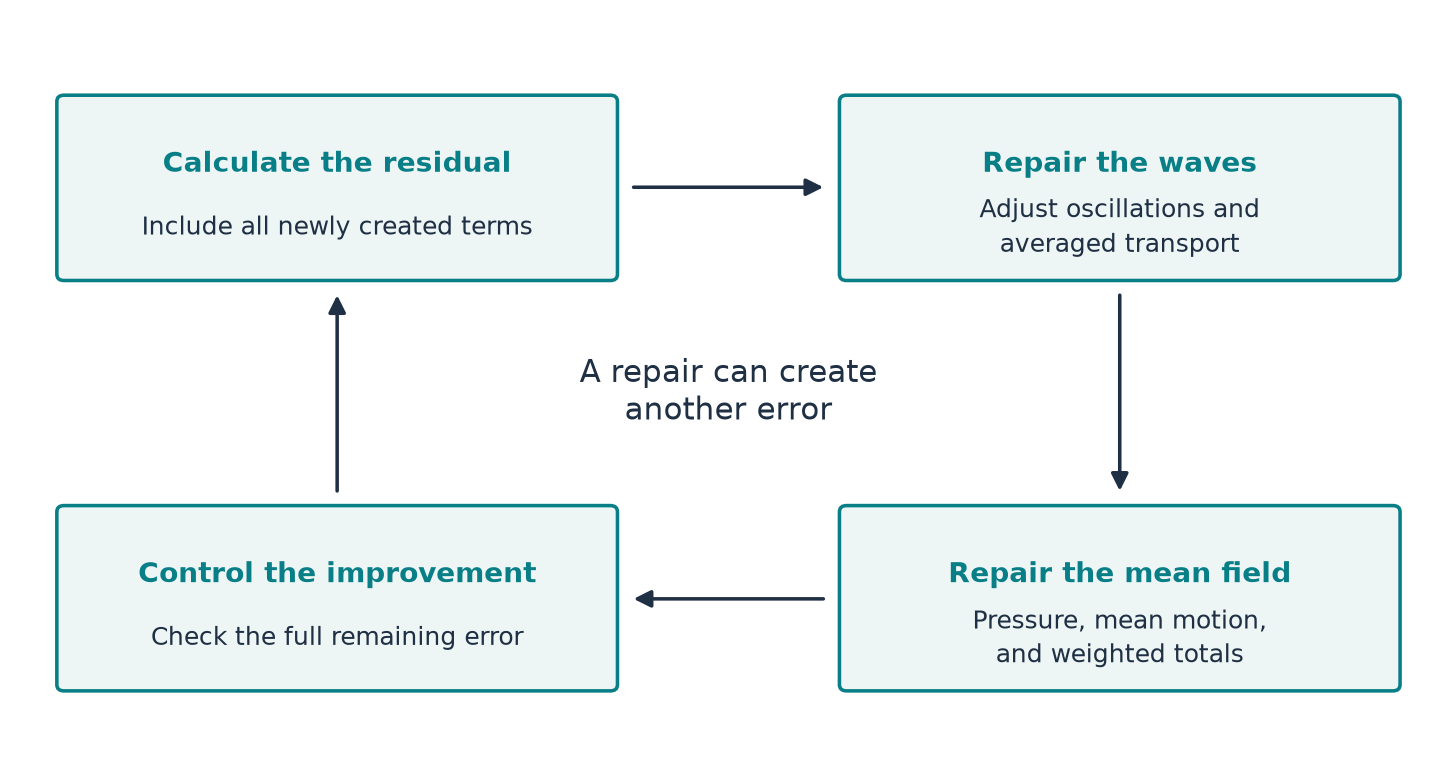
\includegraphics[keepaspectratio,alt={A loop connects calculate all remaining errors, repair waves and average transport, repair mean motion and pressure, restore weighted totals, and calculate again.}]{figures/reader.png}}

}

\caption{\label{fig-cycle}Each repair is followed by a new calculation
of the full mismatch. The stages target different pieces; the diagram
does not claim a measured numerical reduction for the full paper flow.}

\end{figure}%

The point is not merely to make a graph of the residual look small. The
paper needs estimates showing that each cycle improves its behaviour as
the singular point is approached.
\href{https://cdn.openai.com/pdf/32d9f210-8b73-45e0-91bc-82a30aef8a9a/navier-stokes.pdf\#page=15}{Paper,
Proposition 9.6 and Figure 6}

\subsection{An infinite sum can be
finite}\label{an-infinite-sum-can-be-finite}

You know an example of infinitely many additions that stay bounded:

\[
\frac12+\frac14+\frac18+\cdots=1.
\]

After the first term, the missing amount is \(1/2\). After the next, it
is \(1/4\). The remaining tail can be bounded, so the sum has a precise
meaning.

A sequence of fluid corrections needs its own tail estimates. The
geometric series is an analogy for why these estimates matter; the
paper's corrections are not literally the numbers above.

The construction also makes later corrections active only in smaller
neighbourhoods of the singular point. Away from that point, only
finitely many stages are active. Close to it, the estimates control the
remaining tails.

This is how infinitely many stages can define an ordinary smooth field
at every time before blow-up. One cannot infer the result simply from
having computed a few successful stages.

\subsection{A small mismatch can still be too
rough}\label{a-small-mismatch-can-still-be-too-rough}

Picture a road with shallow but very closely spaced bumps. Its height
differs little from a flat road, yet the slope changes rapidly. A car
still notices them.

The force in this problem must be smooth through the singular time. A
force value approaching zero is not enough if its spatial or time
variations behave badly.

The paper's local residual is made \emph{flat} at the singular point: it
and each fixed order of its derivatives vanish faster than every fixed
power of the concentration scale. In ordinary language, the mismatch
must become small with enough control over how it changes.

No new calculation is needed to understand the logical requirement. The
hard analysis supplies the quantitative bounds, including the errors
from cutting off and combining corrections.
\href{https://cdn.openai.com/pdf/32d9f210-8b73-45e0-91bc-82a30aef8a9a/navier-stokes.pdf}{Paper,
Section 9.5 and Equation (3.4)}

\subsection{Turn the flow on gently and confine it
smoothly}\label{turn-the-flow-on-gently-and-confine-it-smoothly}

An abrupt switch creates a sharp change. That would be a poor way to
obtain a smooth force. A \textbf{cutoff} is a smooth transition from one
to zero, like a dimmer rather than an instantaneous switch.

The construction uses such transitions to make the velocity vanish
initially and outside a bounded spatial region. Near the collapsing
centre, the cutoff equals one, so it leaves the essential motion intact.

There is a complication. Multiplying a fluid velocity directly by a
cutoff generally breaks incompressibility. The paper works with a
representation that preserves the ``no accumulation of volume''
condition when the cutoff is applied, and it retains the resulting extra
velocity terms.

You do not need to calculate a vector potential or a curl to understand
their job here: they are a construction tool for keeping
incompressibility exact while restricting where the flow lives. The
extra terms created in the transition region still enter the force
calculation.

The exterior flow has good limiting behaviour away from the singular
point. That allows these transition-region force terms to remain smooth.
Section 10 combines this with the residual estimates near the centre and
extends the force beyond the singular time.
\href{https://cdn.openai.com/pdf/32d9f210-8b73-45e0-91bc-82a30aef8a9a/navier-stokes.pdf}{Paper,
Sections 2.3, 3.5 and 10.1--10.2}

\subsection{Return to the promised
result}\label{return-to-the-promised-result}

The final argument must keep several claims together: increasing
velocity near the chosen point, smoothness before the chosen time,
bounded total energy, zero initial velocity, and a smooth force with
bounded spatial and temporal support.

The paper also uses a comparison argument: another smooth solution with
the same initial data and force, in the stated bounded-energy class,
must agree with the constructed flow before the singular time. That
connects constructing this flow to the claimed failure of a global
smooth continuation in that class.

These are conclusions of the paper's complete estimates. Our cartoons
and isolated computations explain the architecture; they do not
independently establish the theorem.

\subsection{Where this fits in the bigger
picture}\label{where-this-fits-in-the-bigger-picture}

\textbf{The early blocks create the mechanism. The finishing blocks make
it compatible with the exact statement the paper is trying to prove.}
Scheduling limits selected interactions; repeated repair improves the
residual; summation controls the infinitely many stages; localization
and extension give the required smooth force.

You can now return to the \href{../paper-map/article.html}{paper map}
and attach a purpose to every major section. For the separate question
of what a shrinking vortex could mean in a real fluid, continue with
\href{../d1_core_size/article.html}{core size and molecular scales}. The
\href{source-notes.md}{source notes} give the precise locations behind
this overview.




\end{document}
